%===================================== CHAP 4 =================================

\chapter{Implementation}\label{cap_4}

\section{Pipeline}

Write about the system acting as a pipeline.
Still focus on how this was done.

Should following sections in this capter be sections or subsections?

\section{Source data}


%%vise til XML utsnitt, og skrive litt om det. Skrive på en måte så noen kan dra nytte av det senere
\subsection{XML format}


\subsection{XML parsing}


\section{Data retrieval}

%%Parsing XML into relevant data in JSON
\subsection{Wikimedia's markup syntax}
\begin{figure}[h]
\caption{The XML structure used in the XML dump of Wikipedias database}
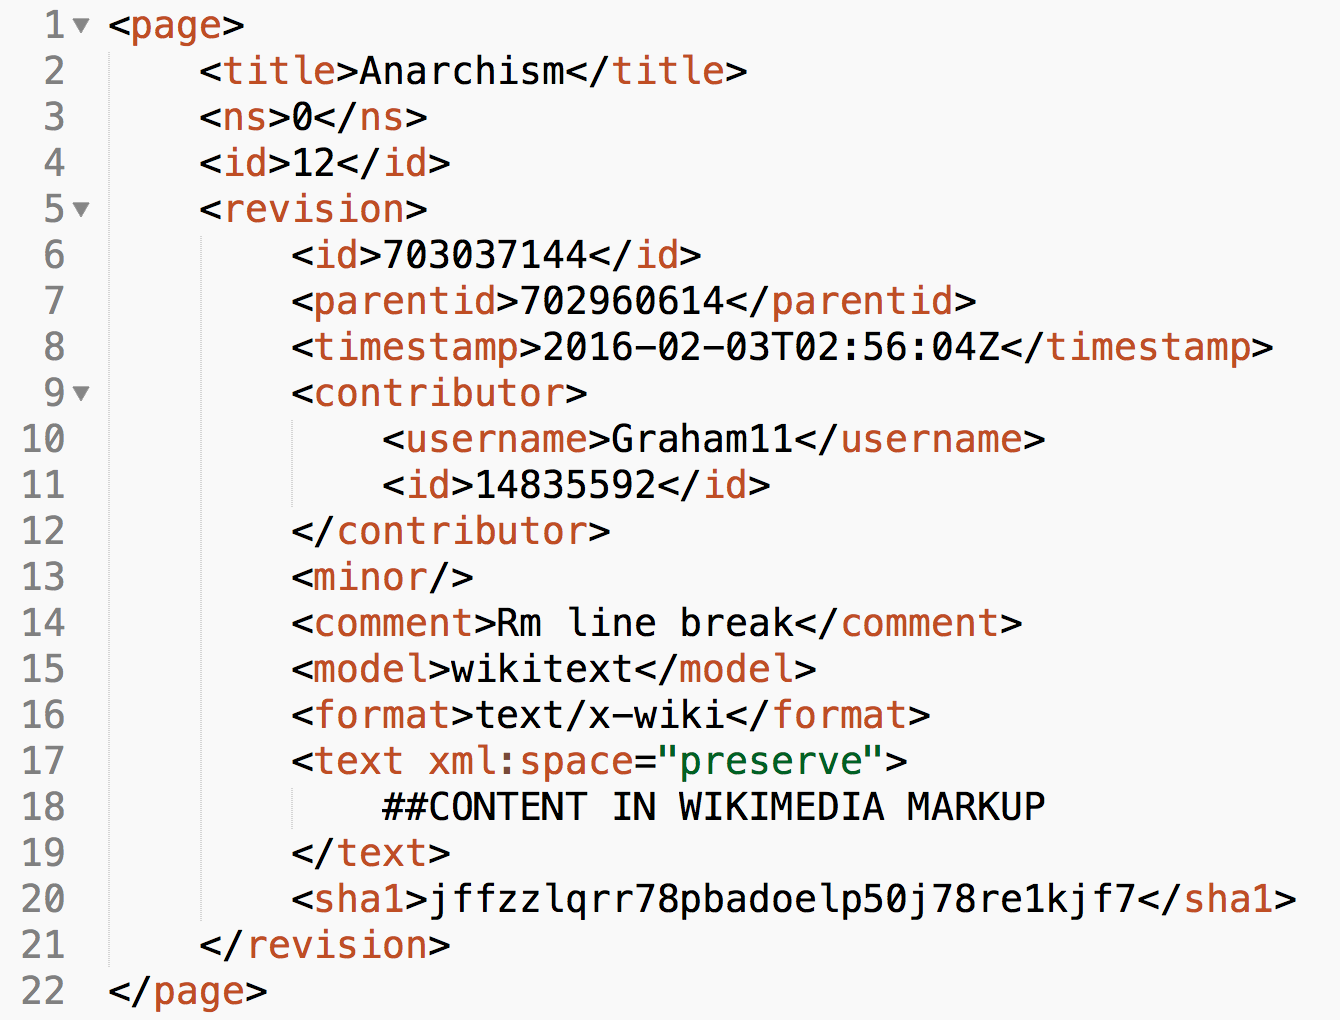
\includegraphics[width=\textwidth]{XMLPage}
\end{figure}

\subsection{Markup parsing}


\section{Data structuring}

%%Inserting the JSON into an sql database
\subsection{Database}

\begin{figure}[h] 
\caption{A simple overview of the database tables and their attributes}
\includegraphics[width=\textwidth]{db_diagram}
\label{fig:db_diagram}
\end{figure}

%% TODO forklare tabellene bedre. Hva de forskjellige termene er i den faktiske wikipedia

Section \ref{custom-pipeline} explains that the source data is fed into the pipeline as a snapshot of Wikipedia at a particular time. The size of the source data is an approximately 50 GB XML-document. Most of this data is not interesting in this project. Therefor the parser excludes most of it before it is structured in the SQL database. 

Figure \ref{fig:db_diagram} displays the tables of the database and the relations between them. If a relevant article is discovered, it is inserted into the \textit{pages} table. The article is found relevant because it contains one or more sections with an example. These sections are then stored in the database with their relation to the article. The categories of the article is also kept, because it will be helpful regarding searching among examples in the finished index.  

The database acts a temporary buffer for the data going into the index. This is helpful because it separates the parsing from the building of the index. This is preferred since the parsing is a very time consuming process, and having it structured in SQL with its meta data helps with showing how successful the parsing was. Most of the meta data is also irrelevant for the index, so only keeping it in the database is beneficial for complexity of the end result.


\section{Indexing data}

Retreviing data fraom the sql database and indexing it.

\section{Searching the data}

Has not been implemented but should maybe be mentioned anyway? Maybe not here?


\cleardoublepage